\documentclass[spanish]{beamer}

\usetheme{default}

\setbeamertemplate{navigation symbols}{}

\usepackage{polyglossia}

\setdefaultlanguage{spanish}
\setotherlanguage[variant=usmax]{english}

\usepackage{tikz}

\usetikzlibrary{automata}

\tikzset{initial text=,node distance=2cm,auto}

\usepackage{fancyvrb}

\DefineShortVerb{\|}
\DefineVerbatimEnvironment{code}{Verbatim}{frame=lines}

\usepackage{fontawesome}

\title{Ahorcado}
\subtitle{Programación funcional imperativa con Elm}
\author{Juan Pedro Villa Isaza}
\institute{Stack Builders}
\date{3 de julio de 2015}

\logo{
\includegraphics[height=0.5cm]{stackbuilders.png}}

\begin{document}

%%%%%%%%%%%%%%%%%%%%%%%%%%%%%%%%%%%%%%%%%%%%%%%%%%%%%%%%%%%%%%%%%%%%%%

\frame{\titlepage}

%%%%%%%%%%%%%%%%%%%%%%%%%%%%%%%%%%%%%%%%%%%%%%%%%%%%%%%%%%%%%%%%%%%%%%

\begin{frame}[fragile]
  \begin{columns}[onlytextwidth,T]
    \begin{column}{.5\textwidth}
      \begin{code}
  ____
  |  |
  |
  |
  |
  |
 ---
      \end{code}
    \end{column}
    \begin{column}{.5\textwidth}
      \begin{code}


 ---------




      \end{code}
    \end{column}
  \end{columns}
\end{frame}

%%%%%%%%%%%%%%%%%%%%%%%%%%%%%%%%%%%%%%%%%%%%%%%%%%%%%%%%%%%%%%%%%%%%%%

\begin{frame}[fragile]
  \begin{columns}[onlytextwidth,T]
    \begin{column}{.5\textwidth}
      \begin{code}
  ____
  |  |
  |
  |
  |
  |
 ---
      \end{code}
    \end{column}
    \begin{column}{.5\textwidth}
      \begin{code}


 ---------

 a


      \end{code}
    \end{column}
  \end{columns}
\end{frame}

%%%%%%%%%%%%%%%%%%%%%%%%%%%%%%%%%%%%%%%%%%%%%%%%%%%%%%%%%%%%%%%%%%%%%%

\begin{frame}[fragile]
  \begin{columns}[onlytextwidth,T]
    \begin{column}{.5\textwidth}
      \begin{code}
  ____
  |  |
  |
  |
  |
  |
 ---
      \end{code}
    \end{column}
    \begin{column}{.5\textwidth}
      \begin{code}


 --a-a----




      \end{code}
    \end{column}
  \end{columns}
\end{frame}

%%%%%%%%%%%%%%%%%%%%%%%%%%%%%%%%%%%%%%%%%%%%%%%%%%%%%%%%%%%%%%%%%%%%%%

\begin{frame}[fragile]
  \begin{columns}[onlytextwidth,T]
    \begin{column}{.5\textwidth}
      \begin{code}
  ____
  |  |
  |
  |
  |
  |
 ---
      \end{code}
    \end{column}
    \begin{column}{.5\textwidth}
      \begin{code}


 --a-a----

 u


      \end{code}
    \end{column}
  \end{columns}
\end{frame}

%%%%%%%%%%%%%%%%%%%%%%%%%%%%%%%%%%%%%%%%%%%%%%%%%%%%%%%%%%%%%%%%%%%%%%

\begin{frame}[fragile]
  \begin{columns}[onlytextwidth,T]
    \begin{column}{.5\textwidth}
      \begin{code}
  ____
  |  |
  |
  |
  |
  |
 ---
      \end{code}
    \end{column}
    \begin{column}{.5\textwidth}
      \begin{code}


 -ua-a-u--




      \end{code}
    \end{column}
  \end{columns}
\end{frame}

%%%%%%%%%%%%%%%%%%%%%%%%%%%%%%%%%%%%%%%%%%%%%%%%%%%%%%%%%%%%%%%%%%%%%%

\begin{frame}[fragile]
  \begin{columns}[onlytextwidth,T]
    \begin{column}{.5\textwidth}
      \begin{code}
  ____
  |  |
  |
  |
  |
  |
 ---
      \end{code}
    \end{column}
    \begin{column}{.5\textwidth}
      \begin{code}


 -ua-a-u--

 e


      \end{code}
    \end{column}
  \end{columns}
\end{frame}

%%%%%%%%%%%%%%%%%%%%%%%%%%%%%%%%%%%%%%%%%%%%%%%%%%%%%%%%%%%%%%%%%%%%%%

\begin{frame}[fragile]
  \begin{columns}[onlytextwidth,T]
    \begin{column}{.5\textwidth}
      \begin{code}
  ____
  |  |
  |  O
  |
  |
  |
 ---
      \end{code}
    \end{column}
    \begin{column}{.5\textwidth}
      \begin{code}


 -ua-a-u--




      \end{code}
    \end{column}
  \end{columns}
\end{frame}

%%%%%%%%%%%%%%%%%%%%%%%%%%%%%%%%%%%%%%%%%%%%%%%%%%%%%%%%%%%%%%%%%%%%%%

\begin{frame}[fragile]
  \begin{columns}[onlytextwidth,T]
    \begin{column}{.5\textwidth}
      \begin{code}
  ____
  |  |
  |  O
  |
  |
  |
 ---
      \end{code}
    \end{column}
    \begin{column}{.5\textwidth}
      \begin{code}


 -ua-a-u--

 o


      \end{code}
    \end{column}
  \end{columns}
\end{frame}

%%%%%%%%%%%%%%%%%%%%%%%%%%%%%%%%%%%%%%%%%%%%%%%%%%%%%%%%%%%%%%%%%%%%%%

\begin{frame}[fragile]
  \begin{columns}[onlytextwidth,T]
    \begin{column}{.5\textwidth}
      \begin{code}
  ____
  |  |
  |  O
  |  |
  |
  |
 ---
      \end{code}
    \end{column}
    \begin{column}{.5\textwidth}
      \begin{code}


 -ua-a-u--




      \end{code}
    \end{column}
  \end{columns}
\end{frame}

%%%%%%%%%%%%%%%%%%%%%%%%%%%%%%%%%%%%%%%%%%%%%%%%%%%%%%%%%%%%%%%%%%%%%%

\begin{frame}[fragile]
  \begin{columns}[onlytextwidth,T]
    \begin{column}{.5\textwidth}
      \begin{code}
  ____
  |  |
  |  O
  |  |
  |
  |
 ---
      \end{code}
    \end{column}
    \begin{column}{.5\textwidth}
      \begin{code}


 -ua-a-u--

 k


      \end{code}
    \end{column}
  \end{columns}
\end{frame}

%%%%%%%%%%%%%%%%%%%%%%%%%%%%%%%%%%%%%%%%%%%%%%%%%%%%%%%%%%%%%%%%%%%%%%

\begin{frame}[fragile]
  \begin{columns}[onlytextwidth,T]
    \begin{column}{.5\textwidth}
      \begin{code}
  ____
  |  |
  |  O
  | /|
  |
  |
 ---
      \end{code}
    \end{column}
    \begin{column}{.5\textwidth}
      \begin{code}


 -ua-a-u--




      \end{code}
    \end{column}
  \end{columns}
\end{frame}

%%%%%%%%%%%%%%%%%%%%%%%%%%%%%%%%%%%%%%%%%%%%%%%%%%%%%%%%%%%%%%%%%%%%%%

\begin{frame}[fragile]
  \begin{columns}[onlytextwidth,T]
    \begin{column}{.5\textwidth}
      \begin{code}
  ____
  |  |
  |  O
  | /|
  |
  |
 ---
      \end{code}
    \end{column}
    \begin{column}{.5\textwidth}
      \begin{code}


 -ua-a-u--

 i


      \end{code}
    \end{column}
  \end{columns}
\end{frame}

%%%%%%%%%%%%%%%%%%%%%%%%%%%%%%%%%%%%%%%%%%%%%%%%%%%%%%%%%%%%%%%%%%%%%%

\begin{frame}[fragile]
  \begin{columns}[onlytextwidth,T]
    \begin{column}{.5\textwidth}
      \begin{code}
  ____
  |  |
  |  O
  | /|
  |
  |
 ---
      \end{code}
    \end{column}
    \begin{column}{.5\textwidth}
      \begin{code}


 -ua-a-ui-




      \end{code}
    \end{column}
  \end{columns}
\end{frame}

%%%%%%%%%%%%%%%%%%%%%%%%%%%%%%%%%%%%%%%%%%%%%%%%%%%%%%%%%%%%%%%%%%%%%%

\begin{frame}[fragile]
  \begin{columns}[onlytextwidth,T]
    \begin{column}{.5\textwidth}
      \begin{code}
  ____
  |  |
  |  O
  | /|
  |
  |
 ---
      \end{code}
    \end{column}
    \begin{column}{.5\textwidth}
      \begin{code}


 -ua-a-ui-

 c


      \end{code}
    \end{column}
  \end{columns}
\end{frame}

%%%%%%%%%%%%%%%%%%%%%%%%%%%%%%%%%%%%%%%%%%%%%%%%%%%%%%%%%%%%%%%%%%%%%%

\begin{frame}[fragile]
  \begin{columns}[onlytextwidth,T]
    \begin{column}{.5\textwidth}
      \begin{code}
  ____
  |  |
  |  O
  | /|\
  |
  |
 ---
      \end{code}
    \end{column}
    \begin{column}{.5\textwidth}
      \begin{code}


 -ua-a-ui-




      \end{code}
    \end{column}
  \end{columns}
\end{frame}

%%%%%%%%%%%%%%%%%%%%%%%%%%%%%%%%%%%%%%%%%%%%%%%%%%%%%%%%%%%%%%%%%%%%%%

\begin{frame}[fragile]
  \begin{columns}[onlytextwidth,T]
    \begin{column}{.5\textwidth}
      \begin{code}
  ____
  |  |
  |  O
  | /|\
  |
  |
 ---
      \end{code}
    \end{column}
    \begin{column}{.5\textwidth}
      \begin{code}


 -ua-a-ui-

 g


      \end{code}
    \end{column}
  \end{columns}
\end{frame}

%%%%%%%%%%%%%%%%%%%%%%%%%%%%%%%%%%%%%%%%%%%%%%%%%%%%%%%%%%%%%%%%%%%%%%

\begin{frame}[fragile]
  \begin{columns}[onlytextwidth,T]
    \begin{column}{.5\textwidth}
      \begin{code}
  ____
  |  |
  |  O
  | /|\
  |
  |
 ---
      \end{code}
    \end{column}
    \begin{column}{.5\textwidth}
      \begin{code}


 gua-a-ui-




      \end{code}
    \end{column}
  \end{columns}
\end{frame}

%%%%%%%%%%%%%%%%%%%%%%%%%%%%%%%%%%%%%%%%%%%%%%%%%%%%%%%%%%%%%%%%%%%%%%

\begin{frame}[fragile]
  \begin{columns}[onlytextwidth,T]
    \begin{column}{.5\textwidth}
      \begin{code}
  ____
  |  |
  |  O
  | /|\
  |
  |
 ---
      \end{code}
    \end{column}
    \begin{column}{.5\textwidth}
      \begin{code}


 gua-a-ui-

 guayaquil


      \end{code}
    \end{column}
  \end{columns}
\end{frame}

%%%%%%%%%%%%%%%%%%%%%%%%%%%%%%%%%%%%%%%%%%%%%%%%%%%%%%%%%%%%%%%%%%%%%%

\begin{frame}[fragile]
  \begin{columns}[onlytextwidth,T]
    \begin{column}{.5\textwidth}
      \begin{code}


    \O/
     |
    / \


      \end{code}
    \end{column}
    \begin{column}{.5\textwidth}
      \begin{code}


¡guayaquil!




      \end{code}
    \end{column}
  \end{columns}
\end{frame}

%%%%%%%%%%%%%%%%%%%%%%%%%%%%%%%%%%%%%%%%%%%%%%%%%%%%%%%%%%%%%%%%%%%%%%

\begin{frame}
  \begin{columns}[onlytextwidth,T]
    \begin{column}{.5\textwidth}
      \begin{figure}
        
\includegraphics[scale=0.4]{elm.png}
      \end{figure}
    \end{column}
    \begin{column}{.5\textwidth}
      Elm es:
      \begin{itemize}
      \item<1->
        Funcional
      \item<1->
        \emph{Puro}
        \begin{itemize}
        \item<1->
          Inmutabilidad
        \item<1->
          Sin efectos secundarios
        \item<1->
          Transparencia referencial
        \end{itemize}
      \item<1-> ...
      \end{itemize}
      \begin{itemize}
      \item<2->
        \emph{Interesante}
      \item<3->
        ¿\alert{Inútil}?
      \end{itemize}
    \end{column}
  \end{columns}
\end{frame}

%%%%%%%%%%%%%%%%%%%%%%%%%%%%%%%%%%%%%%%%%%%%%%%%%%%%%%%%%%%%%%%%%%%%%%

\begin{frame}
  \begin{figure}
    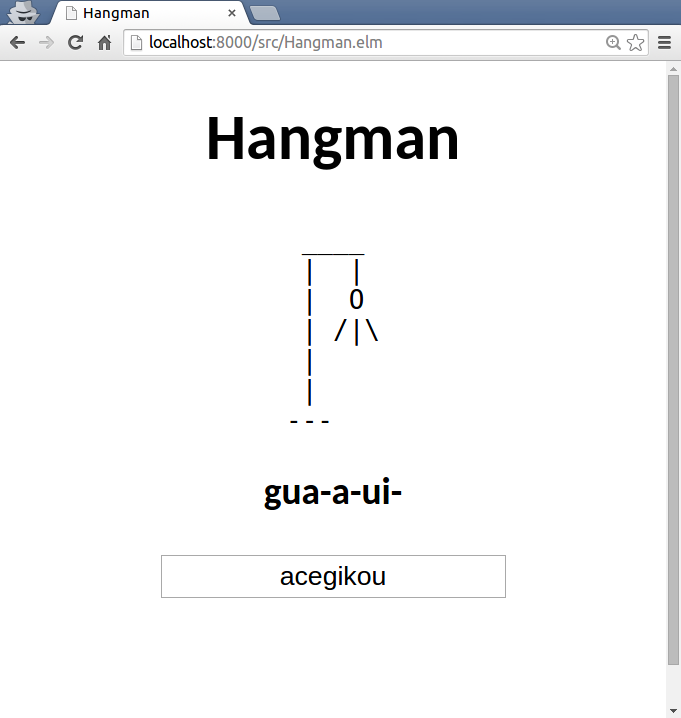
\includegraphics[height=.9\textheight]{elm-hangman-1.png}
  \end{figure}
\end{frame}

%%%%%%%%%%%%%%%%%%%%%%%%%%%%%%%%%%%%%%%%%%%%%%%%%%%%%%%%%%%%%%%%%%%%%%

\begin{frame}<1>[label=quote]
  \begin{quote}
    Los lenguajes de programación funcional son los mejores lenguajes
    de programación imperativa.
  \end{quote}
\end{frame}

%%%%%%%%%%%%%%%%%%%%%%%%%%%%%%%%%%%%%%%%%%%%%%%%%%%%%%%%%%%%%%%%%%%%%%

\begin{frame}[fragile]
  \begin{itemize}
  \item
    Modelo
    \begin{figure}
      \begin{tikzpicture}
        \node [draw] {|[('e',False),('l',False),('m',False)]|};
      \end{tikzpicture}
    \end{figure}
  \item
    Vista
    \begin{figure}
      \begin{tikzpicture}
        \node [state,initial] {|---|};
      \end{tikzpicture}
    \end{figure}
  \item
    Actualización
    \begin{figure}
      \begin{tikzpicture}
        \node [state,initial]   (---)                  {|---|};
        \node [state]           (---a) [right of=---]  {|---|};
        \node [state]           (e--)  [right of=---a] {|e--|};
        \node [state]           (e-m)  [right of=e--]  {|e-m|};
        \node [state,accepting] (elm)  [right of=e-m]  {|elm|};

        \draw [->] (---)  to node [above] {\texttt{a}} (---a);
        \draw [->] (---a) to node [above] {\texttt{e}} (e--);
        \draw [->] (e--)  to node [above] {\texttt{m}} (e-m);
        \draw [->] (e-m)  to node [above] {\texttt{l}} (elm);
      \end{tikzpicture}
    \end{figure}
  \end{itemize}
\end{frame}

%%%%%%%%%%%%%%%%%%%%%%%%%%%%%%%%%%%%%%%%%%%%%%%%%%%%%%%%%%%%%%%%%%%%%%

\begin{frame}[fragile]
  \begin{code}
type alias Model =
  List (Char, Bool)
  \end{code}
\end{frame}

%%%%%%%%%%%%%%%%%%%%%%%%%%%%%%%%%%%%%%%%%%%%%%%%%%%%%%%%%%%%%%%%%%%%%%

\begin{frame}[fragile]
  \begin{code}
init : String -> Model
init word =
  String.foldr (::) [] word
    |> List.map (\letter -> (letter, False))
  \end{code}
\end{frame}

%%%%%%%%%%%%%%%%%%%%%%%%%%%%%%%%%%%%%%%%%%%%%%%%%%%%%%%%%%%%%%%%%%%%%%

\begin{frame}[fragile]
  \begin{code}
type alias Action =
  Char
  \end{code}
\end{frame}

%%%%%%%%%%%%%%%%%%%%%%%%%%%%%%%%%%%%%%%%%%%%%%%%%%%%%%%%%%%%%%%%%%%%%%

\begin{frame}[fragile]
  \begin{code}
update : Action -> Model -> Model
update guess letters =
  let
    match guess (letter, guessed) =
      (letter, guess == letter || guessed)
  in
    List.map (match guess) letters
  \end{code}
\end{frame}

%%%%%%%%%%%%%%%%%%%%%%%%%%%%%%%%%%%%%%%%%%%%%%%%%%%%%%%%%%%%%%%%%%%%%%

\begin{frame}[fragile]
  \begin{code}
view : Signal.Address Action -> Model -> Html
view address model =
  Html.div
    [ ... ]
    [ Html.h1 [] [ Html.text "Hangman" ]
    , Html.h3 [] [ Html.text (toString model) ]
    , Html.input
        [ Html.Events.onKeyPress address Char.fromCode ]
        []
    ]
  \end{code}
\end{frame}

%%%%%%%%%%%%%%%%%%%%%%%%%%%%%%%%%%%%%%%%%%%%%%%%%%%%%%%%%%%%%%%%%%%%%%

\begin{frame}[fragile]
  \begin{code}
toString : Model -> String
toString letters =
  let
    fromLetter (letter, guessed) =
      if guessed then letter else '-'
  in
    List.map fromLetter letters
      |> List.foldr String.cons ""
  \end{code}
\end{frame}

%%%%%%%%%%%%%%%%%%%%%%%%%%%%%%%%%%%%%%%%%%%%%%%%%%%%%%%%%%%%%%%%%%%%%%

\begin{frame}[fragile]
  \begin{code}
main : Signal Html
main =
  StartApp.start
    { model = init "guayaquil"
    , view = view
    , update = update
    }
  \end{code}
\end{frame}

%%%%%%%%%%%%%%%%%%%%%%%%%%%%%%%%%%%%%%%%%%%%%%%%%%%%%%%%%%%%%%%%%%%%%%

\begin{frame}
  \begin{figure}
    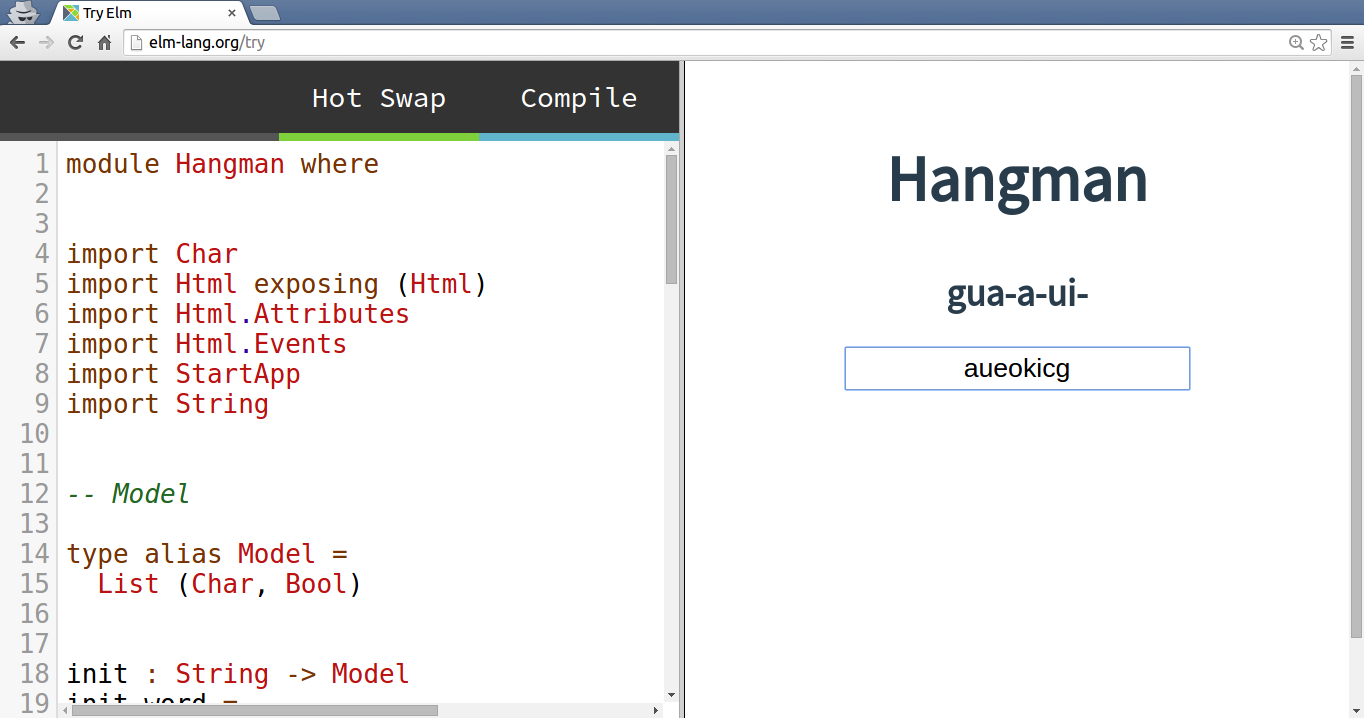
\includegraphics[width=\textwidth]{elm-hangman-2.png}
  \end{figure}
\end{frame}

%%%%%%%%%%%%%%%%%%%%%%%%%%%%%%%%%%%%%%%%%%%%%%%%%%%%%%%%%%%%%%%%%%%%%%

\begin{frame}[fragile]
  \begin{itemize}
  \item
    Modelo
    \begin{figure}
      \begin{tikzpicture}
        \node [draw] {|{[('e',False),('l',False),('m',False)],6}|};
      \end{tikzpicture}
    \end{figure}
  \item
    Vista
    \begin{figure}
      \begin{tikzpicture}
        \node [state with output,initial] {|---| \nodepart{lower} 6};
      \end{tikzpicture}
    \end{figure}
  \item
    Actualización
    \begin{figure}
      \begin{tikzpicture}[state/.style=state with output]
        \node [state,initial] (---) {|---| \nodepart{lower} 6};
        \node [state] (---a) [right of=---] {|---| \nodepart{lower} 5};
        \node [state] (e--)  [right of=---a] {|e--| \nodepart{lower} 5};

        \draw [->] (---)  to node [above] {\texttt{a}} (---a);
        \draw [->] (---a) to node [above] {\texttt{e}} (e--);
      \end{tikzpicture}
    \end{figure}
  \end{itemize}
\end{frame}

%%%%%%%%%%%%%%%%%%%%%%%%%%%%%%%%%%%%%%%%%%%%%%%%%%%%%%%%%%%%%%%%%%%%%%

\begin{frame}[fragile]
  \begin{itemize}
  \item
    \begin{code}
type alias Model =
  { letters : List (Char, Bool)
  , status : Status
  }
    \end{code}
  \item
    \begin{code}
type Status
  = Lost
  | Playing Int
  | Won
    \end{code}
  \end{itemize}
\end{frame}

%%%%%%%%%%%%%%%%%%%%%%%%%%%%%%%%%%%%%%%%%%%%%%%%%%%%%%%%%%%%%%%%%%%%%%

\begin{frame}[fragile]
  \begin{figure}
    \begin{tikzpicture}
      \node (a) at (0,0) {
        \begin{tabular}{c}
          \Huge{\faDesktop}\\\huge{\faKeyboard}
        \end{tabular}
      };
      \node [draw] (c) at (4,4) {
        \begin{tabular}{c}
          Arquitectura Elm:\\|Model|, |view|, |update|
        \end{tabular}
      };
      \draw [->,dotted] (a) -- (0,4) -- (c);
      \draw [->,dotted] (c) -- (4,0) -- (a);
    \end{tikzpicture}
  \end{figure}
\end{frame}

%%%%%%%%%%%%%%%%%%%%%%%%%%%%%%%%%%%%%%%%%%%%%%%%%%%%%%%%%%%%%%%%%%%%%%

\begin{frame}[fragile]
  Distinción clara entre:
  \begin{itemize}
  \item
    Código impuro y código puro
  \item
    Programación imperativa y programación no imperativa
  \end{itemize}
\end{frame}

%%%%%%%%%%%%%%%%%%%%%%%%%%%%%%%%%%%%%%%%%%%%%%%%%%%%%%%%%%%%%%%%%%%%%%

\begin{frame}
  \begin{itemize}
  \item
    Lo mejor de la programación funcional:
    \begin{itemize}
    \item
      Razonamiento ecuacional
    \item
      ...
    \end{itemize}
  \item
    Programación funcional imperativa:
    \begin{itemize}
    \item
      Menos dolores de cabeza
    \item
      ...
    \end{itemize}
  \end{itemize}
\end{frame}

%%%%%%%%%%%%%%%%%%%%%%%%%%%%%%%%%%%%%%%%%%%%%%%%%%%%%%%%%%%%%%%%%%%%%%

\againframe<2>{quote}

%%%%%%%%%%%%%%%%%%%%%%%%%%%%%%%%%%%%%%%%%%%%%%%%%%%%%%%%%%%%%%%%%%%%%%

\end{document}
